% =============================================================================
% TRANSPORT FAILOVER AND HOT SWITCHING
% =============================================================================

\newpage
\section{Transport Failover and Hot Switching}
\label{sec:transport-failover}

This section documents how the STAR gateway automatically detects transport failures, switches between USB CDC and SPI, recovers when a failed transport comes back online, and maintains communication continuity throughout.

\subsection{Architecture Overview}

The gateway's \texttt{TransportManager} (\texttt{internal/manager/manager.go}) orchestrates all failover logic. It maintains exactly \textbf{one active transport} at any time and proxies all \texttt{Send()}/\texttt{Receive()} operations through it. The RX72N firmware is a \textbf{passive listener} --- it does not participate in transport selection decisions.

\vspace{0.3cm}

\noindent\makebox[\textwidth]{%
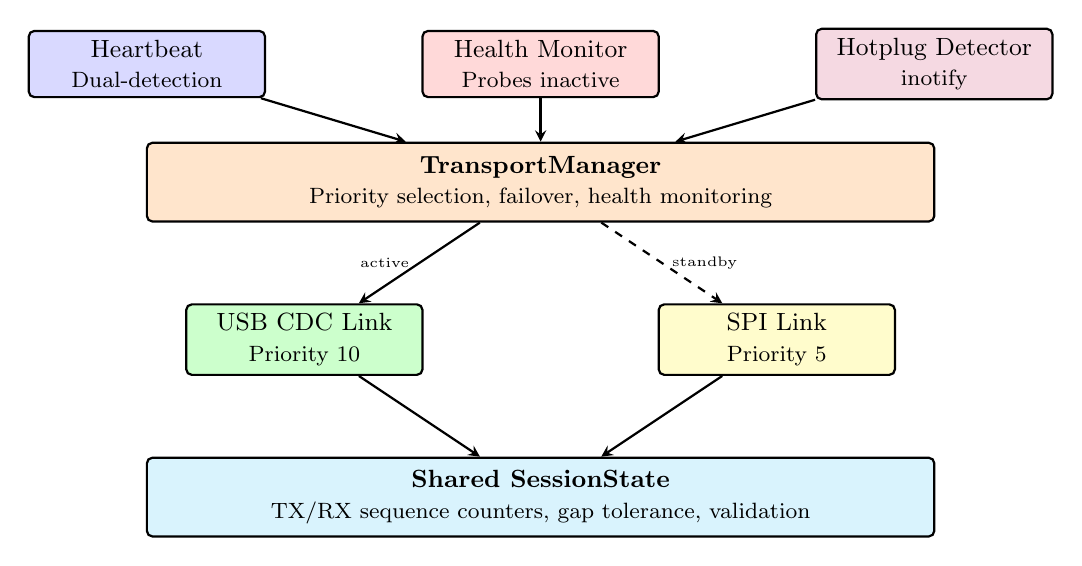
\begin{tikzpicture}[
    font=\small,
    node distance=0.5cm,
    box/.style={draw, thick, rectangle, minimum width=4cm, minimum height=1cm, align=center, rounded corners=2pt},
    smallbox/.style={draw, thick, rectangle, minimum width=3cm, minimum height=0.8cm, align=center, rounded corners=2pt},
    arrow/.style={->, thick, >=stealth},
    dasharrow/.style={->, thick, >=stealth, dashed}
]
    % TransportManager
    \node[box, fill=orange!20, minimum width=10cm] (tm) at (0,0) {\textbf{TransportManager}\\{\footnotesize Priority selection, failover, health monitoring}};

    % Active indicator
    \node[smallbox, fill=green!20] (usb) at (-3,-2) {USB CDC Link\\{\footnotesize Priority 10}};
    \node[smallbox, fill=yellow!20] (spi) at (3,-2) {SPI Link\\{\footnotesize Priority 5}};

    % Subsystems
    \node[smallbox, fill=blue!15] (hb) at (-5,1.5) {Heartbeat\\{\footnotesize Dual-detection}};
    \node[smallbox, fill=red!15] (hm) at (0,1.5) {Health Monitor\\{\footnotesize Probes inactive}};
    \node[smallbox, fill=purple!15] (hp) at (5,1.5) {Hotplug Detector\\{\footnotesize inotify}};

    % Session State
    \node[box, fill=cyan!15, minimum width=10cm] (ss) at (0,-4) {\textbf{Shared SessionState}\\{\footnotesize TX/RX sequence counters, gap tolerance, validation}};

    % Arrows
    \draw[arrow] (tm) -- node[left, font=\tiny] {active} (usb);
    \draw[dasharrow] (tm) -- node[right, font=\tiny] {standby} (spi);
    \draw[arrow] (hb) -- (tm);
    \draw[arrow] (hm) -- (tm);
    \draw[arrow] (hp) -- (tm);
    \draw[arrow] (usb) -- (ss);
    \draw[arrow] (spi) -- (ss);
\end{tikzpicture}%
}

\vspace{0.3cm}

\noindent\colorbox{keyinsightcolor}{\parbox{\dimexpr\linewidth-2\fboxsep}{%
\textbf{Key Insight:} The gateway sends on exactly one transport at a time. It never sends the same command on both USB and SPI simultaneously. The RX72N firmware listens on both channels but the gateway's single-active-transport design means only one will have data at any given moment (except during brief failover transitions).
}}

\subsection{Priority System}

Each transport is registered with a numeric priority. Higher values indicate preferred transports:

\begin{table}[H]
\centering
\caption{Transport Priority Configuration}
\label{tab:failover-priorities}
\begin{tabular}{l c l l}
\toprule
\textbf{Transport} & \textbf{Priority} & \textbf{Role} & \textbf{Rationale} \\
\midrule
USB CDC & 10 & Primary   & Lower latency, hardware CRC, no HARQ overhead \\
SPI     & 5  & Backup    & Always available, full HARQ protection \\
\bottomrule
\end{tabular}
\end{table}

\textbf{Priority rules:}
\begin{enumerate}[leftmargin=1.5em,topsep=4pt,itemsep=2pt]
    \item At startup, the transport with the highest priority that is healthy becomes active.
    \item If the active transport fails, switch to the highest-priority healthy alternative.
    \item If a higher-priority transport recovers, switch back to it (after damping period).
    \item Priority values are constants defined at compile time, not configurable at runtime.
\end{enumerate}

\subsection{Dual-Detection Heartbeat}

The heartbeat system uses two independent mechanisms to detect transport failures. This provides both fast failure detection (implicit) and explicit liveness checking (PING/PONG).

\subsubsection{Implicit Heartbeat (200\,ms Timeout)}

Any valid frame received on a transport resets that transport's implicit heartbeat timer. If no frame arrives within 200\,ms, the transport is considered unhealthy.

\begin{itemize}[leftmargin=1.5em,topsep=4pt,itemsep=2pt]
    \item \textbf{Timer reset:} Every valid frame (COMMAND, RESPONSE, TELEMETRY, PONG, ACK) resets the timer.
    \item \textbf{Timeout:} 200\,ms with no frames $\rightarrow$ mark transport as \texttt{degraded}.
    \item \textbf{No extra traffic:} Piggybacked on existing data flow. In normal operation at 100\,Hz (10\,ms between frames), the implicit timer never fires.
    \item \textbf{Fast detection:} If the USB cable is unplugged mid-stream, detection occurs within 200\,ms.
\end{itemize}

\subsubsection{Explicit Heartbeat (1\,s PING/PONG)}

When the link is idle (no data frames for 1\,second), the gateway sends a PING frame and expects a PONG response within 200\,ms.

\begin{itemize}[leftmargin=1.5em,topsep=4pt,itemsep=2pt]
    \item \textbf{PING interval:} Sent after 1\,second of idle (no other frames sent or received).
    \item \textbf{PONG timeout:} 200\,ms. If no PONG arrives, the transport is marked unhealthy.
    \item \textbf{Purpose:} Detects silent failures where the physical connection exists but the remote device is unresponsive (e.g., firmware crash, watchdog reset).
    \item \textbf{Frame types:} PING = \texttt{0x00}, PONG = \texttt{0x01} (see frame type table in Section~\ref{sec:communication-stack}).
\end{itemize}

\textbf{Why two mechanisms?}
\begin{itemize}[leftmargin=1.5em,topsep=4pt,itemsep=2pt]
    \item \textbf{Implicit} catches failures during active communication (fast: 200\,ms).
    \item \textbf{Explicit} catches failures during idle periods (slower: 1\,s + 200\,ms).
    \item Neither generates unnecessary traffic alone. Combined, they cover all scenarios.
\end{itemize}

\subsection{Health Monitoring}

The \texttt{HealthMonitor} (\texttt{internal/manager/health\_monitor.go}) runs a background goroutine that periodically probes \textbf{inactive} transports to detect when they recover. It does not interfere with the active transport.

\subsubsection{Health Thresholds}

A transport is considered unhealthy if \textbf{any} of the following conditions are met:

\begin{table}[H]
\centering
\caption{Health Monitoring Thresholds}
\label{tab:health-thresholds}
\begin{tabular}{l l l}
\toprule
\textbf{Metric} & \textbf{Threshold} & \textbf{Detection Method} \\
\midrule
Consecutive failures  & $\geq 3$         & Send or receive returns error 3 times in a row \\
Average latency       & $> 200$\,ms      & Exponential moving average of round-trip times \\
Packet loss rate      & $> 10\%$         & Sliding window over recent operations \\
\bottomrule
\end{tabular}
\end{table}

\subsubsection{Probing Inactive Transports}

The health monitor checks inactive transports every 5 seconds (configurable via \texttt{HealthCheckInterval}):

\begin{enumerate}[leftmargin=1.5em,topsep=4pt,itemsep=2pt]
    \item Select all transports that are \textbf{not} the currently active transport.
    \item For each inactive transport, send a PING and wait for PONG.
    \item If PONG received within timeout: mark transport as healthy, record recovery timestamp.
    \item If probe fails: keep transport marked as unhealthy.
    \item If a recovered transport has \textbf{higher priority} than the current active transport, trigger failover (subject to damping window).
\end{enumerate}

\subsection{Failover State Machine}

The \texttt{TransportManager} operates as a state machine with the following states:

\begin{table}[H]
\centering
\caption{Transport Manager States}
\label{tab:tm-states}
\begin{tabular}{l l p{7cm}}
\toprule
\textbf{State} & \textbf{Constant} & \textbf{Description} \\
\midrule
Active USB   & \texttt{StateActiveUSB}   & USB CDC is the active transport, SPI is standby \\
Active SPI   & \texttt{StateActiveSPI}   & SPI is the active transport, USB is unavailable or unhealthy \\
Degraded     & \texttt{StateDegraded}    & Active transport is unhealthy but no better alternative exists \\
Failed       & \texttt{StateFailed}      & No healthy transports available \\
\bottomrule
\end{tabular}
\end{table}

\subsubsection{State Transitions}

\vspace{0.3cm}

\noindent\makebox[\textwidth]{%
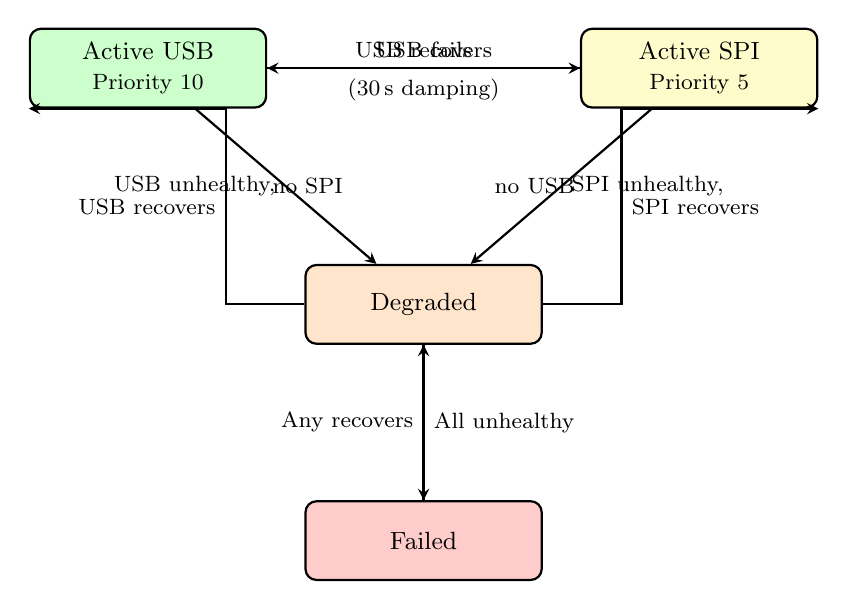
\begin{tikzpicture}[
    font=\small,
    node distance=2.5cm,
    state/.style={draw, thick, rectangle, minimum width=3cm, minimum height=1cm, align=center, rounded corners=4pt},
    arrow/.style={->, thick, >=stealth}
]
    \node[state, fill=green!20] (usb) at (0,0) {Active USB\\{\footnotesize Priority 10}};
    \node[state, fill=yellow!20] (spi) at (7,0) {Active SPI\\{\footnotesize Priority 5}};
    \node[state, fill=orange!20] (deg) at (3.5,-3) {Degraded};
    \node[state, fill=red!20] (fail) at (3.5,-6) {Failed};

    \draw[arrow] (usb) -- node[above, font=\footnotesize] {USB fails} (spi);
    \draw[arrow] (spi) -- node[above, font=\footnotesize] {USB recovers} node[below, font=\footnotesize] {(30\,s damping)} (usb);
    \draw[arrow] (usb) -- node[left, font=\footnotesize] {USB unhealthy,} node[right, font=\footnotesize, xshift=-0.3cm] {no SPI} (deg);
    \draw[arrow] (spi) -- node[right, font=\footnotesize] {SPI unhealthy,} node[left, font=\footnotesize, xshift=0.3cm] {no USB} (deg);
    \draw[arrow] (deg) -- node[right, font=\footnotesize] {All unhealthy} (fail);
    \draw[arrow] (fail) -- node[left, font=\footnotesize] {Any recovers} (deg);
    \draw[arrow] (deg.west) -- ++(-1,0) |- node[left, font=\footnotesize, near start] {USB recovers} (usb.south west);
    \draw[arrow] (deg.east) -- ++(1,0) |- node[right, font=\footnotesize, near start] {SPI recovers} (spi.south east);
\end{tikzpicture}%
}

\subsection{Smart Drain}

When switching away from a transport, the gateway uses ``smart drain'' to handle in-flight frames gracefully:

\begin{itemize}[leftmargin=1.5em,topsep=4pt,itemsep=2pt]
    \item \textbf{Hard failure (IO error, disconnect):} Skip drain entirely. Switch immediately. In-flight frames are lost but speed is critical --- the motor control loop cannot afford a 500\,ms pause.
    \item \textbf{Graceful degradation (high latency, packet loss):} Wait up to 500\,ms for in-flight frames to complete before switching. This avoids losing frames that are nearly delivered.
\end{itemize}

\textbf{Failover timing with smart drain:}

\begin{table}[H]
\centering
\caption{Failover Timing by Failure Type}
\label{tab:failover-timing}
\begin{tabular}{l l l}
\toprule
\textbf{Failure Type} & \textbf{Detection} & \textbf{Total Failover Time} \\
\midrule
USB cable unplugged     & $\sim$200\,ms (implicit timeout) & $< 300$\,ms (no drain) \\
USB device hang         & $\sim$1.2\,s (PING timeout)      & $< 1.5$\,s (no drain) \\
High latency            & $\sim$200\,ms (threshold)        & $< 700$\,ms (500\,ms drain) \\
RX72N firmware crash    & $\sim$1.2\,s (PING timeout)      & $< 1.5$\,s (no drain) \\
\bottomrule
\end{tabular}
\end{table}

\noindent\colorbox{importantcolor}{\parbox{\dimexpr\linewidth-2\fboxsep}{%
\textbf{Important:} The worst-case failover time (1.5\,s) is well within the RX72N's 500\,ms communication watchdog on the \emph{active} transport, but frames from the \emph{standby} transport would arrive before the watchdog fires. The 500\,ms watchdog applies to total communication silence, not to any individual transport.
}}

\subsection{Shared SessionState (Preventing the Handoff Problem)}
\label{subsec:shared-session}

The ``Handoff Problem'' occurs when two transports maintain separate sequence counters:

\begin{enumerate}[leftmargin=1.5em,topsep=4pt,itemsep=2pt]
    \item Gateway sends frames 1--100 over USB (USB sequence = 100, SPI sequence = 0).
    \item USB fails. Gateway switches to SPI.
    \item If SPI has its own counter starting at 0, the RX72N sees sequence ``jump'' from 100 to 0.
    \item The RX72N rejects frame 0 as a duplicate (already seen sequence 0 from USB earlier).
    \item \textbf{Result:} Total communication failure after failover.
\end{enumerate}

\textbf{Solution:} Both transports share a single \texttt{SessionState} object that owns the TX and RX sequence counters:

\begin{lstlisting}[language=Go, caption={Shared SessionState (manager/session.go)}]
type SessionState struct {
    mu         sync.Mutex
    txSequence uint16  // Shared TX counter (both USB and SPI)
    rxSequence uint16  // Shared RX counter (both USB and SPI)
    gapMax     uint16  // Maximum acceptable sequence gap (default: 10)
}

func (s *SessionState) NextTxSequence() uint16 {
    s.mu.Lock()
    defer s.mu.Unlock()
    seq := s.txSequence
    s.txSequence++
    return seq
}
\end{lstlisting}

\textbf{After failover:} Gateway sends frames 1--100 over USB, then frame 101 over SPI. The RX72N sees a continuous sequence regardless of which physical transport delivered it.

\subsubsection{Gap Tolerance}

The shared \texttt{SessionState} accepts sequence gaps of up to 10 frames (\texttt{gapMax = 10}). This handles:

\begin{itemize}[leftmargin=1.5em,topsep=4pt,itemsep=2pt]
    \item \textbf{Rare USB packet loss:} A frame lost during transmission creates a gap of 1. The next frame (sequence $N+1$) is accepted despite the missing $N$.
    \item \textbf{Failover transitions:} During the switch, 1--3 frames may be in-flight on the old transport and never delivered. The new transport picks up at the next sequence number.
    \item \textbf{Duplicate rejection:} Frames with sequences $\leq$ the last accepted sequence are rejected as duplicates (prevents replay).
\end{itemize}

\subsection{USB Hot-Plug Detection}
\label{subsec:hotplug}

The gateway uses Linux \texttt{inotify} to detect USB device attach/detach events in real time, without polling:

\begin{itemize}[leftmargin=1.5em,topsep=4pt,itemsep=2pt]
    \item \textbf{Watch path:} \texttt{/sys/bus/usb/devices} (Linux sysfs)
    \item \textbf{Events:} \texttt{IN\_CREATE} (device attached), \texttt{IN\_DELETE} (device removed)
    \item \textbf{Latency:} Near-instant ($< 50$\,ms from physical plug/unplug to software notification)
    \item \textbf{Filter:} Only reacts to changes matching the RX72N's USB VID/PID (\texttt{045B:0261}, Renesas RX)
\end{itemize}

\textbf{Hot-plug flow:}
\begin{enumerate}[leftmargin=1.5em,topsep=4pt,itemsep=2pt]
    \item USB cable plugged in $\rightarrow$ inotify fires \texttt{IN\_CREATE}.
    \item Hotplug detector opens \texttt{/dev/ttyACM0}, creates USB transport and CDC link.
    \item Registers new transport with \texttt{TransportManager} (priority 10).
    \item If USB has higher priority than current transport $\rightarrow$ switch to USB.
    \item USB cable unplugged $\rightarrow$ inotify fires \texttt{IN\_DELETE}.
    \item Hotplug detector notifies \texttt{TransportManager} $\rightarrow$ immediate failover to SPI.
\end{enumerate}

\subsection{Failback Damping (30-Second Cooldown)}
\label{subsec:failback-damping}

When a previously failed transport recovers, the gateway does \textbf{not} switch back immediately. A 30-second damping window prevents rapid oscillation (``flapping'') between transports:

\begin{itemize}[leftmargin=1.5em,topsep=4pt,itemsep=2pt]
    \item \textbf{Scenario:} USB fails, gateway switches to SPI. USB recovers 2 seconds later.
    \item \textbf{Without damping:} Gateway immediately switches back to USB. If USB is intermittent, it fails again 1 second later. Gateway switches to SPI again. This ``flapping'' disrupts communication.
    \item \textbf{With damping:} Gateway records the USB recovery timestamp. Waits 30 seconds. Only if USB has been continuously healthy for 30 seconds does the gateway switch back.
\end{itemize}

\textbf{Damping parameters:}

\begin{table}[H]
\centering
\caption{Failback Damping Parameters}
\label{tab:damping-params}
\begin{tabular}{l l l}
\toprule
\textbf{Parameter} & \textbf{Value} & \textbf{Description} \\
\midrule
Damping window     & 30\,s       & Minimum healthy duration before failback \\
Health check rate   & 5\,s        & How often inactive transports are probed \\
Recovery condition  & 6 consecutive healthy probes & 6 $\times$ 5\,s = 30\,s of health \\
\bottomrule
\end{tabular}
\end{table}

\subsection{Reset Handshake (Gateway Restart Recovery)}
\label{subsec:reset-handshake}

When the gateway restarts (process crash, reboot, update), the RX72N may still be running with sequence counters at, say, 5000. The restarted gateway's counters start at 0. Without synchronization, the RX72N would reject all frames as out-of-sequence.

\textbf{Three-way reset handshake:}
\begin{enumerate}[leftmargin=1.5em,topsep=4pt,itemsep=2pt]
    \item \textbf{Gateway $\rightarrow$ RX72N:} Send \texttt{RESET} frame (type \texttt{0xFF}).
    \item \textbf{RX72N $\rightarrow$ Gateway:} Respond with \texttt{RESET\_ACK} frame (type \texttt{0xFE}). RX72N resets its TX/RX counters to 0.
    \item \textbf{Gateway:} Receives \texttt{RESET\_ACK}, resets its own SessionState counters to 0.
    \item Both sides are now synchronized at sequence 0. Normal communication resumes.
\end{enumerate}

\textbf{Timeout:} If no \texttt{RESET\_ACK} is received within 500\,ms, the gateway retries the \texttt{RESET} frame (up to 3 times). If all retries fail, the gateway assumes the RX72N is unreachable and enters the \texttt{StateFailed} state.

\noindent\colorbox{importantcolor}{\parbox{\dimexpr\linewidth-2\fboxsep}{%
\textbf{Important:} The reset handshake prevents a ``restart deadlock'' where the gateway cannot communicate because sequences are mismatched, and the RX72N cannot be told to reset because it rejects the out-of-sequence reset frame. The RESET frame type is handled specially by the RX72N --- it is always accepted regardless of sequence number.
}}

\subsection{Firmware Side: Passive Listener}

The RX72N firmware does not participate in transport selection. It is a \textbf{passive listener} that:

\begin{enumerate}[leftmargin=1.5em,topsep=4pt,itemsep=2pt]
    \item Listens on both USB CDC and SPI simultaneously.
    \item Accepts valid frames from either channel (validated by CRC-32 and sequence number).
    \item Does not know or care which transport the gateway considers ``active.''
    \item Routes all received commands through the same callback (\texttt{internal\_frame\_callback}).
    \item Sends telemetry on whichever channel last received a command (implicit response routing).
\end{enumerate}

The \texttt{rx\_comm\_manager\_poll()} function (\texttt{rx\_comm\_manager.c:1317}) polls both channels sequentially every 10\,ms (100\,Hz):

\begin{lstlisting}[language=C, caption={RX72N Dual-Channel Polling}]
rx_err_t rx_comm_manager_poll(rx_comm_manager_t* mgr) {
    /* Poll USB first */
    rx_err_t usb_err = internal_poll_usb(mgr);
    /* Poll SPI second */
    rx_err_t spi_err = internal_poll_spi(mgr);
    /* Process event queue */
    internal_process_event_queue(mgr);
    /* Check heartbeat timers */
    internal_check_heartbeat(mgr);
    return received ? k_rx_ok : k_rx_err_timeout;
}
\end{lstlisting}

\subsection{Timing Summary}

\begin{table}[H]
\centering
\caption{Transport Failover Timing Summary}
\label{tab:failover-timing-summary}
\begin{tabular}{l l}
\toprule
\textbf{Event} & \textbf{Timing} \\
\midrule
Implicit heartbeat timeout      & 200\,ms \\
Explicit PING interval          & 1\,s idle \\
PING/PONG timeout               & 200\,ms \\
Health check interval           & 5\,s \\
Smart drain (graceful)          & up to 500\,ms \\
Smart drain (hard failure)      & 0\,ms (immediate) \\
Failback damping window         & 30\,s \\
Reset handshake timeout         & 500\,ms per attempt, 3 retries \\
RX72N comm watchdog             & 500\,ms \\
USB hot-plug detection           & $< 50$\,ms \\
Worst-case failover (cable pull) & $< 300$\,ms \\
Worst-case failover (silent)     & $< 1.5$\,s \\
\bottomrule
\end{tabular}
\end{table}

\subsection{Cross-References}

\begin{itemize}[leftmargin=1.5em,topsep=4pt,itemsep=2pt]
    \item \textbf{Section~\ref{sec:communication-stack}}: Protocol stack, HARQ details, frame format
    \item \textbf{Section~\ref{sec:dual-channel-arbitration}}: How the RX72N handles simultaneous data on both channels
    \item \textbf{Section~\ref{sec:gateway-architecture}}: Gateway service architecture and directory structure
    \item \textbf{Section~\ref{sec:usb_cdc_protocol}}: USB CDC transport details
    \item \texttt{star-gateway/internal/manager/manager.go}: TransportManager implementation
    \item \texttt{star-gateway/internal/manager/heartbeat.go}: Dual-detection heartbeat
    \item \texttt{star-gateway/internal/manager/health\_monitor.go}: Health probing for inactive transports
    \item \texttt{star-gateway/internal/manager/hotplug\_detector.go}: USB inotify-based hot-plug detection
    \item \texttt{star-gateway/internal/manager/session.go}: Shared SessionState
\end{itemize}
